\documentclass[11pt,letterpaper]{article}
\usepackage[margin=0.86in]{geometry}
\usepackage[T1]{fontenc}
\usepackage[utf8]{inputenc}
\usepackage{lmodern}
\usepackage{xcolor}
\usepackage{tabularx,booktabs,array,longtable}
\usepackage{enumitem}
\usepackage{hyperref}
\usepackage{fancyhdr}
\usepackage{lastpage}
\usepackage{titlesec}
\usepackage{amsmath,amssymb}
\usepackage{microtype}
\usepackage{graphicx}
\usepackage{needspace}
\usepackage{ragged2e}
\definecolor{navy}{HTML}{19334C}
\definecolor{teal}{HTML}{236B82}
\definecolor{soft}{HTML}{EFF5F7}
\definecolor{muted}{HTML}{52616B}
\hypersetup{colorlinks=true,linkcolor=teal,urlcolor=teal}
\titleformat{\section}{\Large\bfseries\color{navy}}{\thesection.}{0.6em}{}
\titleformat{\subsection}{\large\bfseries\color{navy}}{\thesubsection}{0.6em}{}
\titleformat{\subsubsection}{\normalsize\bfseries\color{navy}}{\thesubsubsection}{0.6em}{}
\titlespacing*{\section}{0pt}{15pt}{6pt}
\titlespacing*{\subsection}{0pt}{10pt}{4pt}
\setlength{\parindent}{0pt}
\setlength{\parskip}{4.5pt}
\setlength{\headheight}{15pt}
\renewcommand{\arraystretch}{1.16}
\setlist[itemize]{topsep=3pt,itemsep=2pt,leftmargin=1.4em}
\setlist[enumerate]{topsep=3pt,itemsep=2pt,leftmargin=1.5em}
\pagestyle{fancy}
\fancyhf{}
\fancyhead[L]{\small\color{muted} Applied Machine Learning \textbar{} Cornell Tech}
\fancyhead[R]{\small\color{muted} Human or AI?}
\fancyfoot[C]{\small\color{muted} Page \thepage\ of \pageref{LastPage}}
\renewcommand{\headrulewidth}{0.3pt}
\newcommand{\placeholder}[1]{\par\noindent\textcolor{teal}{\textit{[Your response: #1]}}\par\vspace{0.3em}}
\newcommand{\figplaceholder}[1]{\par\noindent\fcolorbox{teal}{soft}{\parbox[c][1.15in][c]{0.94\linewidth}{\centering\textcolor{muted}{Insert #1 here}}}\par}
\newcommand{\question}[2]{\needspace{4\baselineskip}\par\addvspace{0.45em}\noindent\textbf{#1}\quad #2\par\nobreak\vspace{0.1em}}
\newcommand{\smallnote}[1]{{\small\color{muted}#1}}
\newcolumntype{Y}{>{\RaggedRight\arraybackslash}X}
\begin{document}
\thispagestyle{empty}
\vspace*{0.2in}
{\color{teal}\bfseries CORNELL TECH \textbar{} APPLIED MACHINE LEARNING}\par
\vspace{0.15in}
{\Huge\bfseries\color{navy} Human or AI?}\par
\vspace{0.07in}
{\LARGE\color{navy} Final Technical Report}\par
\vspace{0.17in}

\textbf{Report Template: }\href{https://github.com/sekhari/human-or-ai-submissions}{TEMPLATE}

\textbf{Github Repository Template: }\href{https://github.com/sekhari/human-or-ai-submissions}{REPO}

\textbf{Welcome to the competition!} Your task is to build a machine learning classifier that predicts whether a passage was written by a human or generated by an AI model. You will use a labeled training set, an additional unlabeled set, and a held-out Kaggle test set. The aim is not just a high leaderboard score: we want you to compare methods, design careful experiments, understand generalization, and explain what your results actually show.

You are encouraged to try several approaches. A well-tested logistic regression or support vector machine is just as legitimate as a neural network. The project is designed to be approachable on a laptop; a GPU is \emph{not required} for full credit.

\vspace{0.06in}
\begin{tabularx}{\linewidth}{@{}>{\bfseries}p{1.58in}Y@{}}
Team / members & Divyesh (dt579), Anusha (ar2664), Shenye (sw2486) \\
Kaggle team name & Group Number 30 \\
GitHub PR URL & \url{https://github.com/sekhari/human-or-ai-submissions/pull/4} \\
\end{tabularx}
\vspace{0.06in}
\subsection*{Your data}
\begin{tabularx}{\linewidth}{@{}lrrY@{}}
\toprule
\textbf{File} & \textbf{Rows} & \textbf{Labels} & \textbf{Purpose} \\
\midrule
\texttt{train.csv} & 10,000 & Visible & Supervised model development: 5,000 human (0), 5,000 AI (1) \\
\texttt{unlabeled.csv} & 3,000 & Hidden & Optional input for semi-supervised methods; required experiment \\
\texttt{test.csv} & 3,000 & Hidden & Predict the probability of AI authorship for Kaggle \\
\texttt{train\_starter\_2000.csv} & 2,000 & Visible & Convenient subset of \texttt{train.csv} for quick experiments \\
\bottomrule
\end{tabularx}

\smallnote{The starter data is a subset, not 2,000 additional labeled examples. Passages are approximately 75--350 words, with mean length near 210 words.}

\subsection*{How the test set works}
The test set mixes familiar and unfamiliar writing domains and AI generators, and includes some adversarially modified AI-written passages. You will \emph{not} receive labels, source model names, domain labels, or difficulty memberships for individual test examples. Submit a probability in $[0,1]$ for each test ID, where 1 means AI-generated. Kaggle evaluates submissions using \textbf{area under the ROC curve (AUROC)}. The \textbf{public leaderboard} covers 900 examples (30\%); the \textbf{private leaderboard} covers 2,100 (70\%) and determines the final competition performance score.


\vfill
\newpage
\section{Competition rubric and submission instructions}
\begin{tabularx}{\linewidth}{@{}Y>{\raggedleft\arraybackslash}p{0.85in}@{}}
\toprule \textbf{Component} & \textbf{Points}\\ \midrule
Kaggle private leaderboard performance & 25 \\
Model comparison and selection & 15 \\
Effect of training data size & 10 \\
Learning from unlabeled data & 5 \\
Generalization and error analysis & 20 \\
Open-ended improvements and insights & 15 \\
Code submission and GitHub PR history & 10 \\
\midrule \textbf{Total} & \textbf{100} \\ \bottomrule
\end{tabularx}

\textbf{How to use this document.} Complete the response fields and tables below; insert plots where requested. Keep your answers concise, specific, and supported by actual experiments. Points appear in brackets beside each question; no separate writing-quality grade is assigned.

\textbf{How credit is awarded.} We grade the \emph{quality of the experimental method, evidence, and interpretation}, not whether a proposed idea succeeds. \textbf{Negative results can also earn full credit} when the comparison is valid, the results are reported accurately, and the conclusions are thoughtful. For each question, make clear what you tried, what you measured, and what you learned. Do not invent scores or results.

\textbf{Submit three items:} (1) final Kaggle submission; (2) this completed report as PDF; (3) one GitHub PR link in the course repository, with runnable code, instructions and meaningful commit history. Include the PR link on the title page. Confirm upload locations and deadline time on the course site. The template for the repository is \href{https://github.com/sekhari/human-or-ai-submissions}{here}

\textbf{Compute and models.} Use models and pipelines that you can run and reproduce. Laptop-friendly training is strongly recommended; use of more expensive methods is allowed but not required for full credit. Do not use external LLM APIs to directly label or predict the competition test passages. Use only the supplied labeled dataset for supervised labels; allowed pretrained weights and AI-assisted development should be disclosed.

\textbf{Validation.} For the required controlled experiments, reserve a fixed stratified \textbf{2,000-row validation set} from \texttt{train.csv}, leaving up to 8,000 rows for training. Use the \emph{same} held-out validation set for comparisons and do not tune on test labels. You may retrain your final Kaggle model on all 10,000 labeled examples after selecting your approach. Where possible, document seeds and avoid source/near-duplicate leakage.

\textbf{Kaggle grading (25 points).} Final performance will use the private AUROC, not leaderboard rank. The intended continuous rule is $25\,\mathrm{clip}((A-0.50)/(T-0.50),0,1)$, where $A$ is your private AUROC and $T$ is the announced full-credit threshold. A provisional value of $T=0.90$ is under consideration; the instructors will confirm the fixed threshold before launch. A reference word TF-IDF and logistic regression baseline achieves approximately 0.868 private AUROC.

\section{Team information and model summary}
\question{Q0.1 [0 points].}{List team members and their main contributions.}

Divyesh Thirukonda Gowri Shankar (dt579): Day 1 data audit, model comparison, learning curves and structural-feature experiments. Anusha Ramachandrareddy (ar2664): Day 2 pseudo-labeling and compact-style blend experiments, notebook and measured handoff. Shenye Wang (sw2486): Day 3 integration, split-identity audit, AI-assisted model replay, subgroup/error analysis and report assembly. These are workstream ownership descriptions; AI-assisted execution is disclosed in Q6.3. Each member completed their assigned day; the scope of AI assistance is described in Q6.3.

\question{Q0.2 [0 points].}{Summarize your final approach in 3--5 sentences. What is the overall pipeline from raw text to probability?}

The selected pipeline averages two logistic-regression probabilities with equal weights. One model uses character 3--5-gram TF-IDF with C=3; the other uses word 1--2-gram TF-IDF plus 28 standardized surface/POS features at block weight 0.1, with C=1. Vocabulary, IDF and scaling are learned only from the 8,000 training rows during validation. After selection, both components are refitted on all 10,000 labeled rows and output P(AI) for the 3,000 test IDs. The Day 2 pseudo-label and 11-feature compact blend are preserved as separate experiments, not silently substituted for this configuration.

\question{Q0.3 [0 points].}{Record your final scores (enter private score only once it is revealed).}

\begin{tabularx}{\linewidth}{@{}Yp{2.5in}@{}}\toprule Metric & Score/status \\ \midrule
Validation AUROC (final local refit) & 0.978162 \\
Kaggle public AUROC & 0.91312 (November 9 submission) \\
Kaggle private AUROC & Not yet revealed \\
\bottomrule\end{tabularx}
The November 9 final local refit reproduced Day 1 AUROC 0.978162 and all 3,000 Day 1 test probabilities exactly. Day 3 independently obtained 0.978174; its validation probabilities differ by at most 0.0158745. Even with the pinned Day 3 package versions and matching tagger resource, the local rerun is not byte-identical to Day 3. Q4 retains the Day 3 analysis of the same configuration. The public-test score is lower than validation by 0.065042; distribution shift and repeated validation selection are plausible explanations, not established causes.

\newpage
\section{Model comparison and selection (15 points)}

\textbf{Learning goal:} demonstrate sensible representation choices, comparisons of at least three approaches, appropriate hyperparameter selection, and evidence-based selection of the final classifier.

\question{Q1.1 [3 points].}{How did you preprocess and represent the text? Specify tokenization, normalization, word/character features or embeddings, and any feature extraction choices. Why?}

Word features use lowercase word unigrams/bigrams with the default scikit-learn token rule (at least two word characters), min\_df=2 and a 60,000-feature cap. Character features use lowercase character 3-5 grams, min\_df=3 and an 80,000-feature cap. Both use sublinear term frequency, smoothed IDF and L2 normalization; stop words are retained and no stemming is applied. The final blend also uses 28 style features (21 surface and seven POS), including repetition, formatting and tag proportions. These use original text, training-fitted standardization and weight 0.1 alongside word TF-IDF. POS tags come from the pretrained NLTK English perceptron tagger. All learned preprocessing is fitted only on training rows. The mixture of recipes, news, abstracts and informal posts motivates lexical, subword and structural representations without treating any feature as proof of authorship.

\question{Q1.2 [5 points].}{Which \textbf{three or more} modeling approaches did you try? Keep the labeled validation partition fixed across models.}

The supplied training file contains 10,000 passages with 5,000 labels per class and no blank or exact duplicated passages. We saved one stratified 8,000/2,000 split with seed 20261023, including ordered IDs and input hashes. Both partitions are balanced. The starter file is a subset and was not added. All fitted preprocessing uses only the training partition. The holdout is reused for model selection, so the winning AUROC is a selection estimate, not an unbiased independent test score. The full-corpus audit found no word-trigram Jaccard pairs at or above 0.70, but a few shared openings/moderate-overlap pairs cross the split. We retain the prescribed holdout and report a secondary score excluding eight validation rows that share the normalized first 80 characters or word-trigram Jaccard similarity of at least 0.50 with a training passage. This leaves 1,992 rows (998 human, 994 AI); it does not certify source independence.

\begin{center}\small\begin{tabular}{>{\raggedright\arraybackslash}p{2.8cm}>{\raggedright\arraybackslash}p{3.5cm}rrr}
\toprule
Model & Text representation & Train AUROC & Val. AUROC & Train time \\
\midrule
Logistic regression & Word TF-IDF (1-2 grams) & 0.9998 & 0.9412 & 1.89 s \\
Logistic regression & Character TF-IDF (3-5 grams) & 0.9991 & 0.9708 & 9.00 s \\
ComplementNB & Word TF-IDF (1-2 grams) & 0.9825 & 0.8988 & 1.90 s \\
Calibrated linear SVM & Word TF-IDF (1-2 grams) & 1.0000 & 0.9432 & 1.87 s \\
\bottomrule\end{tabular}\end{center}

The table shows the best setting per representation/classifier combination. The full ten-candidate grid is saved in results/comparison.json. Training times include preprocessing with two numerical-library threads. Logistic regression uses liblinear, max\_iter=2000. SVM probabilities use three seeded training-only sigmoid-calibration folds; those internal folds share the outer-training vocabulary/IDF, but the held-out validation set never enters fitting.

\question{Q1.3 [4 points].}{For at least \textbf{two} approaches, which hyperparameters and candidate values did you try? How did you select the final settings without using Kaggle test labels?}

\begin{center}\small\begin{tabular}{p{4.1cm}p{5cm}p{2.8cm}}
\toprule
Model & Parameters/values searched & Chosen setting \\
\midrule
Word logistic regression & C in \{0.3, 1, 3\} & C=3 \\
Character logistic regression & C in \{0.3, 1, 3\} & C=3 \\
ComplementNB & alpha in \{0.1, 1, 3\} & alpha=1 \\
\bottomrule\end{tabular}\end{center}

Before inspecting any model validation score, we fixed C in \{0.3,1,3\} for word and character logistic regression and alpha in \{0.1,1,3\} for ComplementNB. The calibrated SVM is an additional fixed C=1 comparison. Maximum validation AUROC selects each family winner and the overall Day 1 configuration, with the first listed candidate breaking exact ties. Log loss and source-overlap sensitivity are diagnostics and do not select the model. We did not consult Kaggle scores or hidden labels. All ten candidates are recorded in results/comparison.json, including weaker settings. Within-family choices: word\_lr: C=3.0; char\_lr: C=3.0; word\_nb: alpha=1.0; word\_svm: C=1.0.

\question{Q1.4 [3 points].}{Which approach did you choose for your final submission? Explain using validation performance, computational cost and/or stability. If you later changed the model, explain why.}

We retain the Day 1 equal-weight probability blend of character TF-IDF logistic regression (C=3) and word TF-IDF plus 28 style/POS features with logistic regression (C=1). Its original validation AUROC was 0.978162 versus 0.970756 for character-only, with recorded fitting times 40.54 versus 9.00 seconds. Day 2 tested a different, 11-feature compact-style blend: 0.971276 versus its character baseline 0.970822. It did not reproduce or supersede the 28-feature blend. Day 3 confirmed identical ordered split IDs across days and independently refitted the original recommendation, obtaining 0.978174. Log loss remains worse than character-only, and repeated validation use creates selection optimism. No new blend weights or classification thresholds were tuned for Day 3. Character-only remains the simpler fallback. The final local refit reproduced validation AUROC 0.978162; the Kaggle result is recorded in Q0.3.

\section{Effect of training data size (10 points)}

\textbf{Learning goal:} understand the effect of the number of labeled examples on fitting and generalization. This is an empirical exercise; no formal sample-complexity theory is required.

\question{Q2.1 [4 points].}{Choose one model configuration. Train it with 500, 1,000, 2,000, 5,000 and 8,000 examples sampled from your 8,000-row training partition. Keep the same validation set and hyperparameters.}

Configuration: character TF-IDF (3-5 grams) with logistic regression C=3. We used nested, balanced stratified samples and seed 20261023, refitting vocabulary and IDF at each size. Hyperparameters and all 2,000 validation IDs remained fixed.

\begin{center}\small\begin{tabular}{rrrp{3cm}}
\toprule
Training rows & Training AUROC & Validation AUROC & Notes (optional) \\
\midrule
500 & 1.000000 & 0.875650 & Fit: 0.58 s \\
1,000 & 1.000000 & 0.923034 & Fit: 1.11 s \\
2,000 & 0.999998 & 0.948718 & Fit: 2.19 s \\
5,000 & 0.999608 & 0.965088 & Fit: 5.61 s \\
8,000 & 0.999148 & 0.970755 & Fit: 9.22 s \\
\bottomrule\end{tabular}\end{center}

The 8,000-row curve score differs from the core comparison by 0.000001 because row order differs; the training IDs and configuration are the same.

\question{Q2.2 [3 points].}{Insert a plot of training and validation AUROC versus training-set size.}

\begin{center}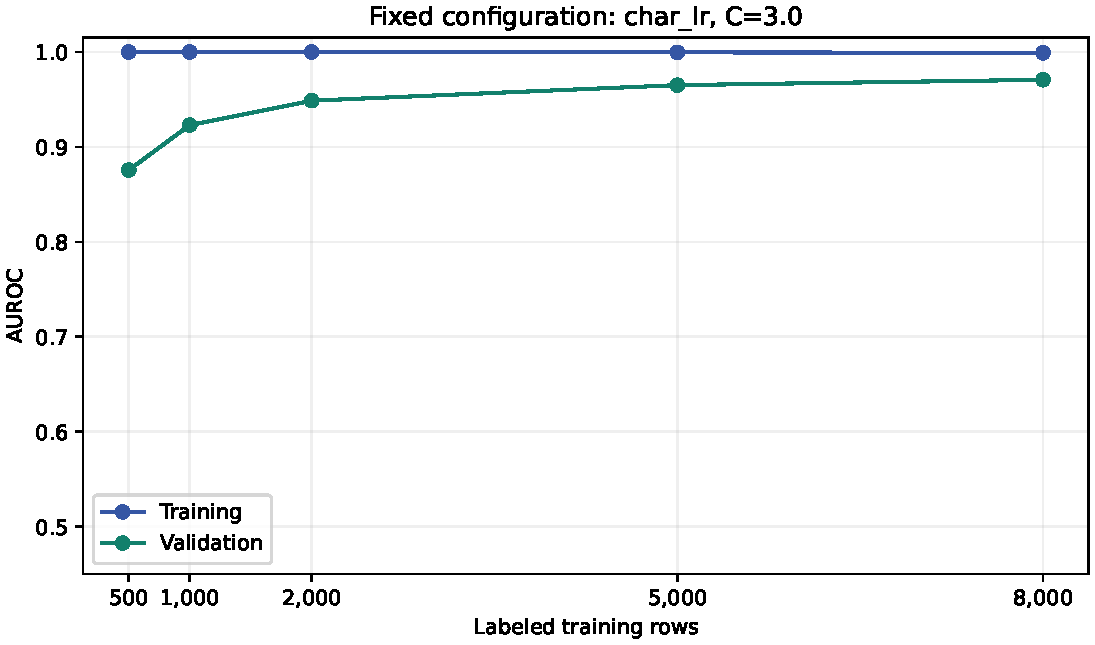
\includegraphics[width=0.92\linewidth]{images/learning_curve.pdf}\end{center}

\question{Q2.3 [3 points].}{What does the curve suggest about overfitting, underfitting, and the value of more labeled examples?}

Validation AUROC changes from 0.8757 at 500 rows to 0.9708 at 8,000 rows (+0.0951); the 5,000-to-8,000 change is +0.0057. The final training-minus-validation gap is +0.0284. The positive gap is consistent with overfitting, although sampling and source variation can contribute. The overall validation increase supports using the available labeled examples for this configuration. Each size uses one nested stratified sample and one seed, with preprocessing refit on that sample. We held hyperparameters and the 2,000 validation IDs fixed. The curve does not quantify sampling variability or justify extrapolating beyond the supplied data. Near-perfect training AUROC offers little evidence of underfitting; the remaining gap suggests a generalization limitation rather than a need for more model capacity.

\section{Learning from unlabeled data (5 points)}
\textbf{Learning goal:} test whether the additional 3,000 unlabeled passages help.
\question{Q3.1 [2 points].}{Describe one method that uses \texttt{unlabeled.csv} (e.g., self-training, confidence-based pseudo-labeling, clustering, or feature learning). How did you prevent validation-label leakage?}

Day 2 trained character 3--5-gram TF-IDF logistic regression (C=3) on the 8,000 labeled training rows, then scored only the supplied 3,000 unlabeled passages. It selected P(AI)$\leq$0.02 as pseudo-human and P(AI)$\geq$0.98 as pseudo-AI, retaining at most 750 from each class in confidence order. The selection contained 95 passages: 12 human and 83 AI. The same model family was refitted on the labeled training rows plus these pseudo-labels, including refitting its vectorizer. Validation examples and labels did not enter selection or fitting. Day 3 compared the saved ID arrays and input hash: both days used the identical ordered training/validation partitions, despite Day 2 recreating rather than loading the manifest.

\question{Q3.2 [2 points].}{Compare against a supervised baseline under the same held-out validation protocol.}

\begin{tabularx}{\linewidth}{@{}Yrr@{}}\toprule Method & Validation AUROC & Log loss \\ \midrule
Supervised character LR & 0.970822 & 0.281667 \\
Character LR plus pseudo-labels & 0.970763 & 0.281552 \\
\bottomrule\end{tabularx}
These are original Day 2 measurements from PR \#1, retained without overwriting. A separate Day 3 replay uses the persisted split and records its own environment and results under \path{results/day3/day2_replay/}.

\question{Q3.3 [1 point].}{Did it help? Give a concrete, evidence-based explanation (including possible noise in pseudo-labels).}

Pseudo-labeling did not improve the competition metric: AUROC decreased by 0.000059. Log loss decreased slightly, but that does not establish a ranking gain. Only 95 of 3,000 unlabeled passages passed the strict confidence rule, and the selected classes were imbalanced (12 human, 83 AI). A small, easy and skewed pseudo-labeled subset may add little new information; incorrect pseudo-labels could reinforce errors. We do not know their true labels, so these are plausible explanations, not measured pseudo-label accuracy. This is a negative result for this one procedure on the reused holdout, not evidence that all uses of unlabeled data fail. Pseudo-labels are not included in the final selected model.

\newpage
\section{Generalization and error analysis (20 points)}
\textbf{Learning goal:} characterize how well the selected model generalizes and where it fails. Use \textbf{labeled validation data}; hidden test labels and hidden domain/generator information are unavailable.

\question{Q4.1 [5 points].}{Compare training and validation AUROC for your final selected model. Is there a gap? What explanations are plausible?}

The independently refitted selected blend achieved training AUROC 0.998926 and validation AUROC 0.978174, a gap of 0.020752. High-dimensional lexical features can fit training-specific wording and formatting, while validation passages contain different combinations. The gap is consistent with overfitting, although sampling/source differences also contribute. The selected holdout was reused for tuning and exploratory choices, so its score may itself be optimistic. Day 1 obtained 0.998927/0.978162 in its recorded environment; Day 3 uses scikit-learn 1.8.0 and the identical NLTK tagger resource. The two prediction vectors differ by up to 0.015874 in probability, despite similar AUROC. This verifies close ranking performance, not exact numerical reproduction or unfamiliar-domain robustness.

\question{Q4.2 [5 points].}{Evaluate performance over at least three text-length bins (define the bins), or another observable subgroup available in your data. Explain why you chose the grouping.}

\begin{tabularx}{\linewidth}{@{}Yrr@{}}\toprule Whitespace-word count & Count & Validation AUROC \\ \midrule
$<$150 words & 380 & 0.968739 \\
150-249 words & 1049 & 0.978170 \\
$\geq$250 words & 571 & 0.986630 \\
\bottomrule\end{tabularx}
Length is observable without hidden domain or generator labels. We fixed simple ranges before inspecting subgroup outcomes and counted words with \texttt{len(text.split())}; ranges are 75--149, 150--249 and 250--350 in this dataset. Human/AI counts are 146/234, 605/444 and 249/322. Short texts rank less well, plausibly because they provide fewer lexical/style cues. At threshold 0.5 the error rates are 9.47\%, 6.96\% and 7.18\%, respectively; ranking and threshold accuracy need not move together. Different genres/class mixtures and unequal sample sizes may explain part of the differences. This observational grouping does not isolate length causally or demonstrate a significant population-level gap.

\question{Q4.3 [5 points].}{Analyze at least \textbf{five false positives and five false negatives} from your held-out validation set. Provide example IDs, predicted probabilities, and short failure hypotheses. Do not paste full passages unless essential.}

Threshold is fixed at P(AI)$\geq$0.5. FP means human predicted AI; FN means AI predicted human. The confusion matrix contains TN=961, FP=39, FN=111 and TP=889. We inspected the five highest-probability FPs and five lowest-probability FNs, selected deterministically with ID tie-breaking. These difficult cases illustrate failures and are not a representative sample of all errors.
\begin{small}\begin{longtable}{@{}p{0.45in}p{0.4in}p{0.73in}p{4.6in}@{}}
\toprule ID & Type & P(AI) & Observed content and possible reason \\ \midrule\endhead
5908 & FP & 0.773076 & Generic corporate-benefits explanation repeats the topic; may resemble generated exposition. \\
483 & FP & 0.756475 & Recipe quantities/instructions may outweigh first-person asides and emphatic capitals. \\
3519 & FP & 0.676570 & Two ingredient lists and repeated cooking steps may resemble generated recipe templates. \\
6921 & FP & 0.675003 & Short board-game post repeats questions; limited context may make its style ambiguous. \\
2349 & FP & 0.618349 & General support advice repeats abstract terms; may resemble generated advice. \\
8309 & FN & 0.139494 & Bank names, dates, acronyms and citation markers may resemble human reference prose. \\
4110 & FN & 0.165551 & Personal grief narrative and short emotional sentences may resemble human posts. \\
5603 & FN & 0.178614 & Colloquial gaming proposal with specialized vocabulary may resemble a human forum post. \\
1036 & FN & 0.178647 & Named entities and chronological biography structure may act as human-reference cues. \\
1602 & FN & 0.195751 & Disambiguation opening and citation markers may act as human-source shortcuts. \\
\bottomrule\end{longtable}\end{small}
These hypotheses follow AI-assisted close reading of the supplied validation passages, not external fact-checking, causal attribution or independent human verification. No full passages are reproduced; detailed observations are saved with the analysis.

\question{Q4.4 [5 points].}{What recurring failure patterns did you identify, and how might you address one of them? Distinguish observed patterns from speculation.}

Among the selected five false negatives, three use reference/biography conventions (8309, 1036, 1602), and two imitate personal or forum-style narration (4110, 5603). Among the selected false positives, two are recipes (483, 3519), while two give general explanation/advice (5908, 2349). These observations show that personal voice, citation formatting and recipe structure can appear on either side of the authorship label. They do not establish the frequency of these patterns among all errors or identify which features caused a prediction. Short passages also have lower subgroup AUROC, but length and genre are confounded. A next experiment could predefine observable recipe/reference-style groups using training data, then compare a fixed model with and without formatting/POS feature families on a fresh evaluation partition. This could test reliance on source shortcuts; it was not performed here and no improvement is claimed. Hidden generator/domain labels are unavailable, and historical or biographical statements were not externally verified.

\newpage
\section{Open-ended improvements and insights (15 points)}
\textbf{Learning goal:} propose and test one improvement beyond the required baseline comparisons. This can be simple: a targeted feature change, alternate regularization scheme, ensemble, different representation, augmentation, or training approach. Sophistication alone does not earn credit.

\question{Q5.1 [3 points].}{What specific question or hypothesis motivated your improvement? What weakness or opportunity did you observe?}

Day 2 asked whether character-level lexical patterns and word-level content plus simple writing-style statistics provide complementary ranking information. Character n-grams capture subword, spelling and punctuation cues, while word n-grams represent local content and the compact style block summarizes length, lexical diversity and formatting. The experiment averaged two independently trained logistic-regression probabilities at a fixed 50/50 weight. This is distinct from Day 1's stronger word/POS-style blend: Day 2 used 11 compact features and no POS tagger. The hypothesis concerns prediction on the fixed validation set; it does not claim that writing style proves authorship or that the components transfer to unfamiliar domains.

\question{Q5.2 [4 points].}{What exactly did you change? Describe the baseline, the new approach and what you held fixed for a fair comparison.}

The baseline was character 3--5-gram TF-IDF (min\_df=3, cap 80,000, sublinear TF, L2 normalization) with logistic regression C=3. The added component used word 1--2-gram TF-IDF (min\_df=2, cap 60,000), 11 standardized style statistics at block weight 0.1, and logistic regression C=1. The statistics cover character/word/sentence counts, length ratios, lexical diversity, punctuation, digits, capitals and newlines. Vocabulary, IDF and scaling were fitted only on the same 8,000 training rows. Predictions were averaged without searching weights. The 2,000 validation IDs, seed, labels and metric were held fixed. Day 3 verified the Day 2 ID arrays against Day 1 rather than assuming equal seeds imply equal partitions.

\question{Q5.3 [4 points].}{What were the measured results?}

\begin{tabularx}{\linewidth}{@{}YrrY@{}}\toprule Configuration & Val. AUROC & Runtime & Difference \\ \midrule
Character LR baseline & 0.970822 & 36.91 s & Log loss 0.281667 \\
Character/compact-style blend & 0.971276 & 37.78 s* & AUROC +0.000454; log loss 0.329447 \\
\bottomrule\end{tabularx}
*Original Day 2 timers are not end-to-end comparable: the baseline includes vectorization plus classifier fitting, but the added 0.87 seconds times only the second classifier fit, excluding word vectorization/style extraction/scaling. It must not be presented as total pipeline overhead. Day 3's portable replay measures both feature extraction and fitting and records separate times. Original metrics are retained for provenance.

\question{Q5.4 [4 points].}{What did you learn? Did the results support the hypothesis? What limits the conclusion, and what would you try next?}

The AUROC increase of 0.000454 provides only weak directional support for complementary ranking information in this compact design. Log loss worsened from 0.281667 to 0.329447, so the result is mixed; log loss alone cannot isolate calibration from discrimination. We did not test repeated training seeds or an independent validation set, and the holdout had already been reused, so the gain should not be described as statistically established or robust. The compact implementation is not an exact reproduction of Day 1's 28-feature POS-based blend, which achieved 0.978162; differences cannot be assigned to one feature without controlled ablations. We retain the reproducible Day 1 blend after an independent Day 3 refit rather than replacing it with the weaker compact variant. Next work would isolate feature families and report complete runtime on fresh evaluation data. Neither this experiment nor the original blend proves generalization to unseen generators or adversarial edits.

\section{Code submission, reproducibility and AI assistance (10 points)}
\textbf{Submission format:} Submit a \textbf{GitHub PR URL} against the course repository. We will inspect the final code and its development history, not just the final snapshot. Do not squash away meaningful intermediate commits before review. Template \href{https://github.com/sekhari/human-or-ai-submissions}{here}.

\question{Q6.1 [5 points].}{Provide the PR URL, the entrypoint for training/evaluation, and the command used to generate \texttt{submission.csv}. State dependencies and random seeds.}

Course-repository PR: \url{https://github.com/sekhari/human-or-ai-submissions/pull/4}. \par Day 3 uses Python 3.12.14 and the tested \path{requirements-day3.txt}; original Day 1 and Day 2 environments remain documented separately. Seed=20261023, two numerical-library threads. From \path{submissions/group-number-30/}, after creating a virtual environment and placing authorized CSVs under \texttt{../../data/}, run:
\begin{small}\begin{verbatim}
python -m pip install -r requirements-day3.txt
python -m nltk.downloader -d ../../data/nltk_data \
  averaged_perceptron_tagger_eng
export NLTK_DATA="$PWD/../../data/nltk_data"
python train.py --train ../../data/train.csv \
  --config results/recommended_config.json --results results
python analyze_day3.py --train ../../data/train.csv
python run_day2.py --data ../../data --out artifacts/day2_replay
python train.py --train ../../data/train.csv \
  --config results/recommended_config.json --full-data \
  --model-out artifacts/final_submission.joblib
python predict.py --test ../../data/test.csv \
  --sample-submission ../../data/sample_submission.csv \
  --model artifacts/final_submission.joblib \
  --out artifacts/submission.csv
\end{verbatim}\end{small}
Use a clean checkout or fresh output paths; scripts intentionally refuse to overwrite recorded training runs. For another verification folder, first copy the saved \texttt{split.json} into it. The POS tagger is a disclosed pretrained annotation resource, not a source of authorship labels. No external LLM API predicts test passages. All text features and models are fitted locally.

\question{Q6.2 [3 points].}{Give two or three examples of changes you made during development. Link to relevant commits or PR discussion and briefly explain what the experiments taught you.}

\begin{enumerate}
\item \href{https://github.com/Divyesh-Thirukonda/human-or-ai-submissions/commit/6d48fe887a7bd20ab3bea83d3a895ffd7383dca4}{Actual-data implementation (6d48fe8)} established data integrity, fixed IDs, four model families and learning curves. Character TF-IDF outperformed word-only features; increasing training size improved the selected model's validation score.
\item \href{https://github.com/Divyesh-Thirukonda/human-or-ai-submissions/commit/c290819a0af34dbf88aa0fb30bf97c2bca39ff72}{Structural blend and resume checks (c290819)} added the original equal blend and stricter artifact checks. The blend improved AUROC but worsened log loss; preserving configurations and predictions made later analysis possible.
\item \href{https://github.com/Divyesh-Thirukonda/human-or-ai-submissions/commit/4545a27a44c33d6b1890244b2f08d65b9f82ff99}{Day 2 experiments} preserved a negative pseudo-label result and a marginal compact-style blend result. Day 3 directly compared split IDs, verified they were identical, distinguished the two style implementations and corrected the runtime interpretation rather than treating every experiment as a success.
\end{enumerate}
Day 3 split auditing and error analysis are preserved in \href{https://github.com/Divyesh-Thirukonda/human-or-ai-submissions/commit/cefec50b94ca9352a6ff2881d89dfce05485aaff}{the course-fork history}. Transferred commits retain original authors and author dates.

\question{Q6.3 [2 points].}{How did you use AI tools (such as Claude, ChatGPT or Copilot) for code, debugging, analysis or writing? What did you verify or modify yourself?}

Codex/ChatGPT assisted with implementation, debugging, experiment execution, validation/error analysis and report drafting. Divyesh completed Day 1, supplied structural hypotheses and directed the actual-data restart. Anusha completed Day 2 and contributed the executed notebook and measured handoff. Shenye completed Day 3 integration, analysis and report assembly. AI-assisted checks compared split IDs and hashes, refitted models, computed subgroup metrics, inspected labeled validation cases and verified output contracts. We do not claim separate manual replication of every result. No external LLM API labeled or predicted test passages, and hidden labels were not retrieved.

\textbf{AI policy.} You may use AI assistants for coding, debugging, explanations, brainstorming, and editing. We expect each team to exercise its own judgment, run experiments, check outputs, and understand its submitted approach. Sending the entire assignment to an AI tool and submitting its unverified output without meaningful involvement does not satisfy the objectives of this project. We will use the PR history, reproducible experiments and report together as evidence of engagement. \emph{Commit counts and the presence of AI-generated code are not themselves grading criteria.} Do not fabricate results or retrieve hidden test labels.


\section*{Final submission checklist}
\begin{itemize}[label=$\square$]
\item Final probabilities submitted to Kaggle and selected for the final leaderboard score; public AUROC 0.91312.
\item Completed report assembled for the Gradescope Kaggle Competition submission.
\item Course-repository PR linked on the title page and in Q6.1.
\item Code and dependencies recreate final predictions (within reasonable numerical tolerance).
\item Relevant experiments and seed/configuration details are recorded.
\item AI-use disclosure is complete; hidden labels were not retrieved externally.
\end{itemize}


\end{document}
